\documentclass{hainanuthesis}

\newcommand{\overbar}[1]{\mkern1.5mu\overline{\mkern-1.5mu#1\mkern-1.5mu}\mkern1.5mu}
\newcommand{\overbari}[1]{\,\overline{\!{#1}}}
\usepackage{subcaption}
\usepackage{algorithm2e}

\addbibresource{articles.bib}

\title{推荐算法研究及实现}
\author{张奥星}
\id{20181682310040}
\grade{2018级}
\faculty{理学院}
\department{数学系}
\major{信息与计算科学}
\teacher{黄萍}

\begin{document}
% \maketitle
\makecover{}

\begin{abstract}
    近年来,
    尤其是在COIVID-19的影响下,
    游戏产业愈发地繁荣.
    同时,
    游戏的数量也越来越多,
    如何从海量的游戏内容当中获取到用户喜爱的游戏,
    成为了游戏产业当中越来越重要的一项议题.

    本文介绍了融合了FM、
    Word2Vec以及神经网络相关技术的一种新型游戏推荐技术,
    以期对Steam游戏进行相关的推荐.
    主要是将稀疏数据进行嵌入之后分别交由FM处理和直接输出,
    对于标签数据则使用Word2Vec进行Tag2Vec的学习,
    与进行嵌入后的稀疏数据以及稠密数据连接后
    交由深度学习模块进行训练.
    考虑到计算性能以及防止过拟合,
    各全连接层之间均使用ReLU作为激活函数,
    最终使用二分类交叉熵损失(BCE)作为损失函数.
    具体的训练模型设计详见\cref{fig:model}.

    经过实验表明本文的模型具有一定的可行性以及有效性,
    最终给出了该模型后续所面临的困难以及接下来的研究方向.
    \keywords{FM;Word2Vec;深度学习;推荐系统;电子游戏}
\end{abstract}

\newpage

\begin{abstract}[en]
    These years,
    especially under the influence of COVID-19,
    more and more video games are springing up.
    How to recommend users' favorite game is becoming
    more and more important.

    This thesis mainly introduce a new recommendation technology,
    including FM, Word2Vec and deep learning.
    The tech is designed for vedio games of Steam,
    a game platform.
    Firstly,
    putting the sparse data into the embedding layer,
    then putting into FM layer.
    Secondly,
    putting the tags into Word2Vec machine and
    contact the result with dense data and
    the result of embedding layer.
    Finally,
    make sure all of the data can be trained by
    the deep learning machine.
    To avoid over-fitting,
    we choose ReLU between the full connection layer,
    or linear layer.
    What's more,
    BCE is the loss function.
    This design can also be learnt in figure 4.

    The model is proved available and validated.
    At the end of this thesis,
    we pointed out the difficulty and
    the direction of the future for further research.
    \keywords[en]{FM; Word2Vec; Deep learning; recommendation system; video games} % chktex 13
\end{abstract}

\newpage
\tableofcontents
\newpage

\section{绪论}

\subsection{研究背景与意义}

随着21世纪互联网的高速发展,
数据的产生与获取也越来越方便,
根据相关研究表明\cite{arnevonseeTotalDataVolume2021},
2021年的数据总量被认为是79ZB,
在2022年,全球数据总量将可能达到97ZB。

网络的迅速发展所带来巨大讯息的同时,
对于普通人来说信息过载的问题也将日趋严重。
因此,
如何建立一个有效的数据分类系统成为了一个日益重要的议题。
对于游戏领域,% TODO Steam数据相关参考文献
以目前最大的游戏应用商店Steam来说,
2020年一年所发布的新游戏已经达到了10000部,
月活用户更是超过1亿,
而且仍有增长的趋势。
因此,
不可避免地需要一种快速、
有效的推荐系统来给每位用户推荐其所偏好的游戏。

\subsection{国内外研究现状}

\subsubsection{国内研究现状}

国内学者对于游戏推荐领域兴趣似乎并不算大,
主要的有俞东进教授及其团队\cite{yuJiYuYinShiFanKuiShuJuDeGeXingHuaYouXiTuiJian2018}以及沙静等人\cite{shaJiYuYinShiFanKuiDeGeXingHuaYouXiTuiJianFangFa2021}基于隐式反馈的游戏推荐系统,
薛梦婷\cite{xieJiYuZhongWenPingLunQingGanQingXiangXingFenXiDeShouYouTuiJianYanJiu2017}基于评论情感倾向性的手游推荐系统,
陈耀旺\cite{chenJiYuShenDuXueXiDeGeXingHuaWangBaYouXiTuiJian2019}等人基于深度学习的游戏推荐系统。
其余学者则多集中在算法的实现方面,
例如使用KNN、
DNN等算法。

相较于国内游戏推荐系统领域的研究匮乏,
其余领域的推荐系统研究则相对较为充分。
例如冯兴杰等人\cite{fengJiYuPingFenJuZhenYuPingLunWenBenDeShenDuTuiJianMoXing2020}基于评分矩阵和评论文本所设计的深度推荐系统,
何蓉\cite{heJiYuJuanJiShenJingWangLuoDeYinLeTuiJianXiTong2019}所提出的基于CNN的音乐推荐系统,
以及吕亚珉\cite{luJiYuFMYuDQNJieHeDeShiPinTuiJianSuanFa2021}等人基于FM和DQN的视频推荐算法等等。

\subsubsection{国外研究现状}

国外学者对游戏推荐系统的研究主要有Gong等人\cite{gongHybridRecommenderSystem2020}提出的混合过滤的Steam游戏推荐系统,
Wang\cite{kangSelfAttentiveSequentialRecommendation2018}等人提出的自我注意的序列化推荐系统以及Pathak\cite{pathakGeneratingPersonalizingBundle2017}等人对于生成Steam游戏合集的推荐系统的研究等等。
而对近似领域的推荐系统的研究则多集中于使用深度学习领域的相关工具,
例如Zhou\cite{zhouCNNRNNBasedIntelligent2021}等人基于CNN、
RNN的媒体推荐系统,
Sahoo\cite{sahooDeepRecoDeepLearning2019}等人基于深度学习的协同过滤推荐系统,
甚至有Wang\cite{wangAdversarialTrainingBasedMean2020}等人基于对抗训练的贝叶斯个性化排序推荐系统等。

\subsection{论文主要研究内容}

由于游戏推荐方面包含用户的游玩时间、
游戏评论与打分以及游戏标签等多种信息,
因此特征分解、
评论情感分析、
深度学习等算法均可用于游戏推荐系统当中。

\subsection{论文组织结构}


\section{游戏推荐算法简介}

自上世纪90年代中叶协同过滤算法的提出\cite{adomaviciusNextGenerationRecommender2005},
使得推荐系统作为一门独立的学科被世人广泛且深入的研究.
在此之后工业界和学术界都提出了一些新的推荐系统的算法.
经过长期的发展,
已经可以给出推荐算法的形式化定义:
令$C$表示为用户集合,
$S$作为所有可作为推荐项目的集合.
在实际的应用生产环境中,
集合$C$和集合$S$都具有相当大的规模.
定义效用函数$u$来计算项目$s$对用户$c$的有用程度,
即$u:C\times S\rightarrow R$.
其中$R$是一个全序集合(即一定范围内的非负整数或实数).
因此,
对每个用户$c\in C$,
我们期望选出项目$s'\in S$使得可以最大化用户的效用.
形式化表达如下:
\begin{equation}
    \forall c\in C,\; s_c'=\arg \max_{s\in S} u(c,s)
\end{equation}

传统的推荐算法通常被分类为以下几种类型\cite{canoHybridRecommenderSystems2017}:
基于内容的推荐、
基于协同过滤的推荐、
统计推荐、
基于知识的推荐、
混合推荐。

\subsection{基于内容的推荐}

基于内容的推荐是较早使用的推荐算法,
其核心思想在于给用户推荐与过去相比较为相似的项目.
即通过对用户已经拥有过的或者评分过的项目的元数据特征进行提取,
计算出用户的偏好,
之后计算用户与项目的相似度并根据相似度的大小进行排序,
排序的结果作为最终的推荐结果.

基于内容的推荐主要依赖于用户的偏好与项目的特征,
不需要其他用户的相关信息,
有效的避免了数据的稀疏性问题,
同时也解决了新项目的冷启动问题.
但是,
基于内容的推荐对特征提取的要求较高,
也很难衡量推荐项目的优劣性,
对于新用户或历史记录较少的用户而言也不够友好,
很难对其进行有效的推荐.

\subsection{基于协同过滤的推荐}

协同过滤算法是Goldberg等人\cite{goldbergUsingCollaborativeFiltering1992}
在1992年提出的一种推荐算法.
其目前为推荐算法当中较为主流的研究方向,
同时也是应用较为广泛的推荐算法.

协同过滤算法主要可以分为基于用户的协同过滤与基于项目的协同过滤.
基于用户的协同过滤主要为
给用户推荐与其偏好较为相似的用户所喜爱的项目,
相似地,
基于项目的协同过滤则主要为
给用户推荐与其喜欢的项目相似的项目.
即依据用户的历史行为偏好计算用户间的相似度(基于用户的协同过滤)
或项目间的相似度(基于项目的协同过滤),
利用用户的历史行为偏好预测用户未来可能表示偏好的项目进行推荐.

\subsection{统计推荐}

统计推荐使用年龄、
性别、
学历等统计数据,
来为用户打上不同的标签.
这种方案可以很好的解决冷启动问题.
然而,
在当今环境下,
由于在线隐私政策,
很难收集到足够多的统计数据来进行足够好的推荐.
但是统计推荐仍然被用来结合其他推荐算法来获得更好的推荐结果.

\subsection{基于知识的推荐}

基于知识的推荐(KBF)
使用关于用户和项目的知识来得知哪种项目满足用户的需求,
并且生成相应的结果\cite{burkeKnowledgeBasedRecommenderSystems2000}.
KBF可以用于推荐用户购买较少的复杂项目(例如汽车、房子等),
并且表示用户(或价格)的重要限制\cite{felfernigConstraintbasedRecommenderSystems2008}.
在这种拥有较少的用户交互数据的系统中使用协同过滤算法或
基于内容的推荐不够现实.

\subsection{混合推荐}

在现实情况下,
单一的推荐算法往往不能很好的解决实际的问题,
因此,
为了充分利用相关数据,
发挥各种推荐算法的优势,
将两种或多种推荐算法组合起来的推荐技术则被称为混合推荐技术.
常用的混合推荐方式有加权型、
分级型、
瀑布型、
合并型、
特征组合型、
特征递增型、
融入其他因素推荐等等.
下文将对一些常见的组合策略进行介绍\cite{heJiYuJuanJiShenJingWangLuoDeYinLeTuiJianXiTong2019}.

\subsubsection{加权型}

加权型将独立的两个或多个推荐算法的算法通过加权相结合,
并将其作为最终的推荐结果.
通过比较用户的评分与算法预测结果的差异进行权重调整.
对于任意用户$u$,
其对项目$i$的推荐度公式为:
\begin{equation}
    f(u,i)=\sum_{j=1}^n\alpha_j f_j(u,i)
\end{equation}

其中$f_j(u,i)$为不同的推荐算法,
$\alpha_j$为不同推荐算法所对应的权重.
加权型推荐精度较高,
但是权重系数调整相对困难,
较为消耗计算资源,
因此实际应用中使用较少.

\subsubsection{分级型}

分级型通过将不同推荐算法的推荐结果进行层次划分,
其次在相应的场景中选用可信度较高的算法推荐,
最后采用其余算法进行递补推荐,
其公式为:
\begin{equation}
    f(u,i)=\sum_{j=1}^n\beta_j(u,i)f_j(u,i)
\end{equation}

其中$f_j(u,i)$为不同推荐算法,
$\beta_j(u,i)$为相应场景中的对应方法的优劣层级.
分级型相对适合进行TopN类型推荐,
且能兼顾推荐的结果的质量与数量.

\subsubsection{瀑布型}

瀑布型通过将推荐算法视为不同粒度的过滤器,
并将前一个推荐算法的输出作为下一个推荐算法的输入,
通过逐步筛选候选结果以得到高精确度的结果,
其公式为:
\begin{equation}
    f(u,i)=g\left(\sum_{j=1}^n\lambda_j f_j(u,i)\right)
\end{equation}

其中$g(\cdot)$为外层推荐算法,
$\sum_{j=1}^n\lambda_j f_j(u,i)$为前一级推荐结果,
$\lambda_j$代表前一级权重.
通常在设计时,
会将便于计算、
较低区分度的推荐算法放在前一级,
以节省计算资源.
通常瀑布型算法在待推荐项目和所需推荐结果数量相差较大时使用.

\subsubsection{合并型}

合并型采用同时使用
多种推荐方法进行推荐并给出各自的推荐结果以及推荐理由
的方案,
以供用户参考.
该方法的推荐结果较为全面,
种类丰富,
有利于培养用户的新偏好.


\section{Word2Vec词嵌入模型简介}

Word2Vec是一种比较流行的词嵌入的方法,
通过将单词转换为定长的向量以方便进行计算。
相对于One-Hot编码来说,
没有了过于稀疏的问题,
同时也可以更好地表达词与词之间的相似或类比关系。

Word2Vec包含有两个模型,
即跳元模型\cite{mikolovDistributedRepresentationsWords2013}
(Skip-gram)
与连续词袋模型\cite{mikolovEfficientEstimationWord2013}
(Continuous Bag of Words),
模型结构如\cref{fig:Word2Vec}所示。

\begin{figure}[!htbp]
    \centering
    \includegraphics[width=0.8\textwidth]{images/Word2Vec.pdf}
    \caption{Word2Vec模型}\label{fig:Word2Vec}
\end{figure}

\subsection{跳元模型}

假设一个单词序列$W = \left\{w_1, w_2, w_3, \ldots, w_T\right\}$,
中心词为$w_t$,
上下文窗口为$2$。
则给定中心词$w_t$,
生成上下文词$w_{t-2}, w_{t-1}, w_{t+1}, w_{t+2}$的条件概率为:
\begin{equation}
    \label{eq:con}
    P(w_{t-2}, w_{t-1}, w_{t+1}, w_{t+2}|w_t)
\end{equation}

若上下文词是在给定中心词的情形下满足条件独立性,
则\cref{eq:con}可以改写为:
\begin{equation}
    P(w_{t-2}|w_t)P(w_{t-1}|w_t)P(w_{t+1}|w_t)P(w_{t+2}|w_t)
\end{equation}

令$\mathbf{v}_{w_t}\in\mathbb{R}^d$和
$\mathbf{u}_{w_t}\in\mathbb{R}^d$
表示$w_t$分别作为中心词和上下文词时的两个$d$维向量。
给定中心词$w_I$,
生成的上下文词$w_O$
的条件概率可以通过softmax函数定义:
\begin{equation}
    P\left(w_O|w_I\right) = \frac{\exp\left(\mathbf{u}_{w_O}^T\mathbf{v}_{w_I}\right)}{\sum_{w_t\in W}\exp\left(\mathbf{u}_{w_t}^T\mathbf{v}_{w_I}\right)}
\end{equation}

由于跳元模型是依据条件概率所构建的,
因此我们可以通过极大似然估计来作为模型优化方向,
即:
\begin{equation}
    \frac{1}{T}\sum^T_{t=1}\sum_{-c\leqslant j\leqslant c, j\neq 0}\log P\left(w_{t+j}|w_t\right)
\end{equation}

其中$c$为上下文窗口的大小。

\subsection{连续词袋模型}

连续词袋模型存在多个上下文词,
故需要在计算条件概率时对上下文词向量进行平均。
即令$\mathbf{v}_{w_t}\in\mathbb{R}^d$和
$\mathbf{u}_{w_t}\in\mathbb{R}^d$
表示$w_t$分别作为中心词和上下文词时的两个$d$维向量。
给定上下文词$w_{O_1}, w_{O_2}, \ldots, w_{O_{2c}}$
生成任意中心词$w_I$的条件概率可以表示为:
\begin{equation}
    P\left(w_I|w_{O_1}, \ldots, w_{O_{2c}}\right) = \frac{\exp\left(\frac{1}{2c}\mathbf{v}_I^T\left(\mathbf{u}_{O_1}+\cdots+\mathbf{u}_{O_{2c}}\right)\right)}{\sum_{w_t\in W}\exp\left(\frac{1}{2c}\mathbf{v}_{w_t}\left(\mathbf{u}_{O_1}+\cdots+\mathbf{u}_{O_{2c}}\right)\right)}
\end{equation}

由此,
连续词袋模型的损失函数可以定义为:
\begin{equation}
    -\sum_{t=1}^T\log P\left(w_t|w_{t-c}, \ldots, w_{t-1}, w_{t+1}, \ldots, w_{t+c}\right)
\end{equation}

\subsection{计算加速}

由于softmax计算的特性,
需要对词表中的每一项都进行计算,
由此可能会造成梯度的计算过于复杂,
影响模型的训练效率。
因此,
我们将引入两种近似训练方法:
负采样和分层softmax。
由于两种模型的相似性,
本文仅以跳元模型为例进行说明。

\subsubsection{噪声对比估计NCE}

NCE是Gutmann等人在2010年\cite{gutmannNoisecontrastiveEstimationNew2010}
处理非归一化模型时提出的一种参数估计原理,
以简化对归一化因子的计算。

假设集合$U=\left(\mathbf{u}_1, \ldots, \mathbf{u}_{2T}\right)$是集合
$X$和$Y$的并集,
令数据集$X$的元素个数为$T_d$,
噪声集$Y$的元素个数为$T_n$,
且给其中元素$u_t$定义标签为:
\begin{equation}
    C_t = \left\{
    \begin{aligned}
         & 1 \quad \text{if} \; \mathbf{u}_t \in X \\
         & 0 \quad \text{if} \; \mathbf{u}_t \in Y
    \end{aligned}
    \right.
\end{equation}

由于数据$\mathbf{x}$服从的概率密度函数$p_d\left(.\right)$未知,
不妨令$p_d\left(.\right)=p_m\left(.;\theta\right)$,
由此可以得到:
\begin{equation}
    p\left(\mathbf{u}|C=1;\theta\right) = p_m\left(\mathbf{u};\theta\right) \quad p\left(\mathbf{u}|C=0\right)=p_n\left(\mathbf{u}\right)
\end{equation}

先验分布为:
\begin{equation}
    \begin{aligned}
         & P\left(C=1\right)=\frac{T_d}{T_d+T_n} \\
         & P\left(C=0\right)=\frac{T_n}{T_d+T_n}
    \end{aligned}
\end{equation}

则根据全概率公式有:
\begin{equation}
    \begin{aligned}
        P\left(\mathbf{u}\right) & =P\left(\mathbf{u}|C=1;\theta\right)P\left(C=1\right)+P\left(\mathbf{u}|C=0\right)P\left(C=0\right) \\
                                 & =p_m\left(\mathbf{u};\theta\right)\frac{T_d}{T_d+T_n}+p_n\left(\mathbf{u}\right)\frac{T_n}{T_d+T_n}
    \end{aligned}
\end{equation}

再根据贝叶斯公式有:
\begin{equation}
    \begin{aligned}
        P\left(C=1|\mathbf{u};\theta\right) & =\frac{P\left(\mathbf{u}|C=1;\theta\right)P\left(C=1\right)}{P\left(\mathbf{u}\right)}                                 \\
                                            & =\frac{p_m\left(\mathbf{u};\theta\right)}{p_m\left(\mathbf{u};\theta\right)+\frac{T_n}{T_d}p_n\left(\mathbf{u}\right)}
    \end{aligned}
\end{equation}

则类别$C_t$的对数似然函数为:
\begin{equation}
    \label{eq:C_tL}
    \begin{aligned}
        L\left(\theta\right) & =\sum_{t=1}^{T_d+T_n}\left[C_t\ln P\left(C_t=1|\mathbf{u}_t;\theta\right)+\left(1-C_t\right)\ln P\left(C_t=0|\mathbf{u}_t\right)\right]        \\
                             & =\sum_{t=1}^{T_d}\ln\left[P\left(C=1|\mathbf{x}_t;\theta\right)\right]+\sum_{t=1}^{T_n}\ln\left[1-P\left(C=1|\mathbf{y}_t;\theta\right)\right]
    \end{aligned}
\end{equation}

由于\cref{eq:C_tL}与交叉熵函数的相似性,
我们可以使用逻辑回归来对模型进行学习,
从而利用相关算法达到简化计算的目的。

\subsubsection{负采样NEG}

负采样实际上是NEC的一种特殊情况,
即使$\frac{T_n}{T_d}p_n\left(\mathbf{u}\right)=1$。
把给定中心词$w_I$,
生成的上下文词$w_O$被认为是由\cref{eq:sigma}
建模的概率事件。
\begin{equation}
    \label{eq:sigma}
    \begin{aligned}
        P\left(D=1|w_I,w_O\right) & = \sigma\left(\mathbf{u}_O^T\mathbf{v}_I\right) \\
        \sigma(x)                 & =\frac{1}{1+\exp(-x)}
    \end{aligned}
\end{equation}

同理,
可以得出相应的对数损失函数。
% TODO 此处应算出相应的损失函数

\section{因子分解机简介}

因子分解机(Factorization Machines,FM)
是由Rendle等人于2010年提出的一种基于矩阵分解的
一种机器学习算法。
其主要将支持向量机(SVM)的优势与因子分解模型相结合,
旨在对极为稀疏的数据进行处理。

总的来说,FM的优势主要在于\cite{rendleFactorizationMachines2010}:
\begin{itemize}
    \item FM可以在SVM所不能处理的及其稀疏的场景下进行参数估计
    \item FM的计算复杂度是线性的,使得FM对大型数据集的计算性能较好
    \item FM在通用场景下拥有较好的表现
\end{itemize}

FM在提出之后获得了大量的关注,
同样地,
也衍生出了许多的变体。
比如Guo等人于2017年提出的DeepFM模型\cite{guoDeepFMFactorizationMachineBased2017},
Juan等人于2016年提出的FFM模型\cite{juanFieldawareFactorizationMachines2016},
He等人于2017年提出的NFM模型\cite{heNeuralFactorizationMachines2017}
等。

\subsection{FM原理}

FM模型的二阶公式为:
\begin{equation}
    \hat{y}(\mathbf{x})=w_0+\sum_{i=1}^n w_i x_i+\sum_{i=1}^n\sum_{j=i+1}^n\langle\mathbf{v}_i,\mathbf{v}_j\rangle x_i x_j
\end{equation}

模型中的参数应当有:
\begin{equation}
    w_0\in\mathbb{R}, \mathbf{w}\in\mathbb{R}^n, \mathbf{V}\in\mathbb{R}^{n\times k}
\end{equation}

其中$\langle\cdot,\cdot\rangle$为两$k$阶向量的点积:
\begin{equation}
    \langle\mathbf{v}_i,\mathbf{v}_j\rangle=\sum_{f=1}^k v_{i,f}\cdot v_{j,f}
\end{equation}

$\mathbf{v}_i$是矩阵$\mathbf{V}$的第$i$个$k$阶变量。
$k\in\mathbb{N}_0^+$为定义了因子维度的一个超参数。

对于二阶FM而言,
$w_0$为全局偏置量,
$w_i$则为第$i$个变量的权重,
$\hat{w}_{i,j}=\langle\mathbf{v}_i,\mathbf{v}_j\rangle$
为第$i$和第$j$个变量的互作用。

\subsection{FM模型计算优化}

显然根据定义,
FM模型的计算复杂度为$O(kn^2)$,
其对于大规模数据的计算不够友好,
较为消耗计算资源,
因此需要对其进行优化。

对于模型定义中的后半部分,可以得出:
\begin{equation}
    \begin{aligned}
          & \sum_{i=1}^{n} \sum_{j=i+1}^{n}\left\langle\mathbf{v}_{i}, \mathbf{v}_{j}\right\rangle x_{i} x_{j}                                                                                                         \\
        = & \frac{1}{2} \sum_{i=1}^{n} \sum_{j=1}^{n}\left\langle\mathbf{v}_{i}, \mathbf{v}_{j}\right\rangle x_{i} x_{j}-\frac{1}{2} \sum_{i=1}^{n}\left\langle\mathbf{v}_{i}, \mathbf{v}_{i}\right\rangle x_{i} x_{i} \\
        = & \frac{1}{2}\left(\sum_{i=1}^{n} \sum_{j=1}^{n} \sum_{f=1}^{k} v_{i, f} v_{j, f} x_{i} x_{j}-\sum_{i=1}^{n} \sum_{f=1}^{k} v_{i, f} v_{i, f} x_{i} x_{i}\right)                                             \\
        = & \frac{1}{2} \sum_{f=1}^{k}\left(\left(\sum_{i=1}^{n} v_{i, f} x_{i}\right)\left(\sum_{j=1}^{n} v_{j, f} x_{j}\right)-\sum_{i=1}^{n} v_{i, f}^{2} x_{i}^{2}\right)                                          \\
        = & \frac{1}{2} \sum_{f=1}^{k}\left({\left(\sum_{i=1}^{n} v_{i, f} x_{i}\right)}^{2}- \sum_{i=1}^{n} v_{i, f}^{2} x_{i}^{2}\right)
    \end{aligned}
\end{equation}

经过上述变换之后模型的计算复杂度将为$O(kn)$。

\section{神经网络相关技术简介}

\subsection{M-P 神经元模型}

如\cref{fig:M-P}所示,
即为M-P神经元模型.
神经元通过接收来自其他$n$个神经元的输入信号,
通过带权重的连接进行传递,
神经元接收到的总输入值与神经元的阈值进行比较,
然后通过激活函数进行处理以产生输出\cite{zhouzhihuaJiQiXueXi}.

\begin{figure}[!htbp]
    \centering
    \includegraphics[width=.6\textwidth]{images/M-P_nn_model.pdf}
    \caption{M-P 神经元模型}\label{fig:M-P}
\end{figure}

激活函数通常使用 Sigmoid 函数和 ReLU 函数:

\begin{equation}
    \label{eq:sigmoid}
    \begin{aligned}
        Sigmoid\left(x\right) = \frac{1}{1+e^{-x}} \\
        ReLU\left(x\right) = \max\left\{0, x\right\}
    \end{aligned}
\end{equation}

其函数图像如\cref{fig:active-func}所示.

\begin{figure}
    \centering
    \begin{minipage}[b]{0.45\textwidth}
        \centering
        \includegraphics[width=0.95\textwidth]{images/Sigmoid.pdf}
        \subcaption{Sigmoid}
        \label{fig:sigmoid}
    \end{minipage}
    \begin{minipage}[b]{0.45\textwidth}
        \centering
        \includegraphics[width=0.95\textwidth]{images/ReLU.pdf}
        \subcaption{ReLU}
        \label{fig:ReLu}
    \end{minipage}
    \caption{多图并排示例}
    \label{fig:active-func}
\end{figure}

\subsection{优化算法}

通常我们会引入损失函数来衡量
神经网络的预测结果和真实结果之间的差距。
一旦拥有了损失函数,
我们便尽可能的使其结果尽可能小来进行尽可能准确的预测,
因此我们便可以使用优化算法来最小化损失。
在神经网络中常用的优化算法有:
梯度下降算法、
随机梯度下降算法、
小批量随机梯度下降算法、
动量法、
AdaGrad算法、
RMSProp算法、
Adadelta算法、
Adam算法等等。
受限于篇幅限制,
本文将着重介绍较为常用的梯度下降算法的实现---
反向传播算法与Adam算法。

\subsubsection{反向传播算法}

由于多层网络的学习能力通常要强于单层感知机,
因此,
需要一种更加强大的算法.
最常用的就是反向传播算法(BP算法),
其不仅可以用于多层前馈神经网络,
同样可以用于诸如递归神经网络等其余类型的网络.
通常情况下“BP 神经网络”指使用 BP 算法训练的多层前馈神经网络.

假定一个前馈神经网络具有$d$个输入神经元,
$l$个输出神经元,
$q$个隐层神经元,
其中输出层第$j$个神经元的阈值为$\theta_j$,
隐层第$h$个神经元的阈值为$\gamma_h$.
记输入层第$i$个神经元与隐层第$h$个神经元的连接权为$v_{ih}$,
隐层层第$h$个神经元与输出层第$j$个神经元的连接权为$w_{ih}$.
记隐层第$h$个神经元接收到的输入为$\alpha_h=\sum_{i=1}^dv_{ih}x_i$,
输出层第$j$个神经元的输出为$\beta_j=\sum_{h=1}^{q}{w_{hj}b_h}$,
$b_h$为隐层第$h$个神经元的输出.
假设隐层和输出层都使用 Sigmoid 函数.

对训练例$\left(\mathbf{x}_k, \mathbf{y}_k\right)$,
假定输出为$\hat{\mathbf{y}}_k=\left(\hat{y}_1^k, \hat{y}_2^k, \ldots, \hat{y}_l^k\right)$,
即:

\begin{equation}
    \label{eq:yjk}
    \hat{y}_j^k = f\left(\beta_j-\theta_j\right)
\end{equation}

则均方误差为:

\begin{equation}
    \label{eq:mse}
    E_k=\frac{1}{2}\sum_{j=1}^l{\left(\hat{y}_l^k-y_j^k\right)^2}
\end{equation}

根据\cref{eq:mse},
以目标的负梯度方向对参数进行调整.
给定学习率$\eta$,
有:

\begin{equation}
    \Delta w_{hj}=\eta\frac{\partial{E_k}}{\partial{w_{hj}}}
\end{equation}

\begin{equation}
    \label{eq:partial}
    \frac{\partial{E_k}}{\partial{w_{hj}}}=\frac{\partial{E_k}}{\partial{\hat{y}_j^k}}\cdot\frac{\partial{\hat{y}_j^k}}{\partial{\beta_j}}\cdot\frac{\partial{\beta_j}}{\partial{w_{hj}}}
\end{equation}

由$\beta$的定义可以得出:

\begin{equation}
    \label{eq:b}
    \frac{\partial \beta_j}{\partial w_{hj}} = b_h
\end{equation}

对于\cref{eq:sigmoid}中 Sigmoid 来说,
有:

\begin{equation}
    f^{\prime}\left(x\right) = f\left(x\right)\left(1-f\left(x\right)\right)
\end{equation}

于是根据\cref{eq:yjk}和\cref{eq:mse},
有:

\begin{equation}
    \label{eq:g}
    \begin{aligned}
        g _ { j } & = - \frac { \partial E _ { k } } { \partial \hat { y } _ { j } ^ { k } } \cdot \frac { \partial \hat { y } _ { j } ^ { k } } { \partial \beta _ { j } } \\
                  & = - ( \hat { y } _ { j } ^ { k } - y _ { j } ^ { k } ) f ^ { \prime } ( \beta _ { j } - \theta _ { j } )                                                \\
                  & = \hat { y } _ { j } ^ { k } ( 1 - \hat { y } _ { j } ^ { k } ) ( y _ { j } ^ { k } - \hat { y } _ { j } ^ { k } )
    \end{aligned}
\end{equation}

把\cref{eq:g}和\cref{eq:b}代入\cref{eq:partial},
即可得出 BP 算法中关于$w_{ij}$的更新公式:

\begin{equation}
    \label{eq:whj}
    \Delta w_{hj} = \eta g_jb_h
\end{equation}

同理可得:

\begin{align}
    \Delta\theta_j                   & = -\eta g_j   \\
    \label{eq:vih}\Delta v_{ih}      & = \eta e_hx_i \\
    \label{eq:gammah}\Delta \gamma_h & = -\eta e_h
\end{align}

\cref{eq:vih}和\cref{eq:gammah}中:

\begin{equation}
    \label{eq:e}
    \begin{aligned}
        e _ { h } & = - \frac { \partial E _ { k } } { \partial b _ { h } } \cdot \frac { \partial b _ { h } } { \partial \alpha _ { h } }                                                                                \\
                  & = - \sum _ { j = 1 } ^ { l } \frac { \partial E _ { k } } { \partial \beta _ { j } } \cdot \frac { \partial \beta _ { j } } { \partial b _ { h } } f ^ { \prime } ( \alpha _ { h } - \gamma _ { h } ) \\
                  & = \sum _ { j = 1 } ^ { l } w _ { h j } g _ { j } f ^ { \prime } ( \alpha _ { h } - \gamma _ { h } )                                                                                                   \\
                  & = b _ { h } ( 1 - b _ { h } ) \sum _ { j = 1 } ^ { l } w _ { h j } g _ { j }
    \end{aligned}
\end{equation}

可以得到计算的算法如\cref{alg:nn}所示\cite{zhouzhihuaJiQiXueXi}.

\begin{algorithm}
    \KwIn{训练集$D=\left\{(x_k, y_k)\right\}^m_{k=1}$; 学习率$\eta$.}
    在$(0, 1)$范围内随机初始化网络中所有链接权和阈值\;
    \Repeat{达到停止条件}{
        \ForAll{$(\mathbf{x}_k, \mathbf{y}_k) \in D$}{
            根据当前参数和\cref{eq:yjk}计算当前样本的输出$\hat{\mathbf{y}}_k$\;
            根据\cref{eq:g}计算输出层神经元的梯度项$g_j$\;
            根据\cref{eq:e}计算隐层神经元的梯度项$e_h$\;
            根据\cref{eq:whj}~--\cref{eq:gammah}更新连接权$w_{hj}$,$v_{ih}$与阈值$\theta_j$,$\gamma_h$
        }
    }
    \KwOut{连接权与阈值确定的多层前馈神经网络}
    \caption{反向传播算法}
    \label{alg:nn}
\end{algorithm}

\subsubsection{Adam算法}

随着深度学习技术的不断发展,
BP算法对于优化速度等方面逐渐不能满足于训练的需要,
使用随机梯度下降算法比仅仅使用梯度下降算法更加有效,
AdaGrad算法对于稀疏梯度的处理更加有效\cite{duchiAdaptiveSubgradientMethods2011},
RMSProp算法在在线和非平稳环境下表现更好\cite{tielemanLecture5rmspropDivide2012}。
Adam算法结合了以上算法的优点,
其具体实现参照\cref{alg:adam}\cite{kingmaAdamMethodStochastic2017}。

\begin{algorithm}
    \KwData{$\alpha$:步长}
    \KwData{$\beta_1,\beta_2\in [0,1)$:非负加权参数}
    \KwData{$f(\theta)$:随机过程函数}
    \KwData{$\theta_0$:初始参数矢量}
    $m_0\leftarrow0$(初始化梯度动量)\;
    $v_0\leftarrow0$(初始化梯度的二阶矩)\;
    $t\leftarrow0$(初始化时间步长)\;
    \While{$\theta_t$不收敛}{
        $t\leftarrow t+1$\;
        $g_{t} \leftarrow \nabla_{\theta} f_{t}\left(\theta_{t-1}\right)$(计算当前梯度)\;
        $ m_{t} \leftarrow \beta_{1} \cdot m_{t-1}+\left(1-\beta_{1}\right) \cdot g_{t} $(更新当前梯度的动量)\;
        $ v_{t} \leftarrow \beta_{2} \cdot v_{t-1}+\left(1-\beta_{2}\right) \cdot g_{t}^{2} $(更新当前梯度的二阶矩)\;
        $ \widehat{m}_{t} \leftarrow m_{t} /\left(1-\beta_{1}^{t}\right) $(标准化梯度的动量)\;
        $ \widehat{v}_{t} \leftarrow v_{t} /\left(1-\beta_{2}^{t}\right) $(标准化梯度的二阶矩)\;
        $ \theta_{t} \leftarrow \theta_{t-1}-\alpha \cdot \widehat{m}_{t} /\left(\sqrt{\widehat{v}_{t}}+\epsilon\right) $(更新参数)\;
    }
    \KwOut{$\theta_t$}
    \caption{Adam算法}
    \label{alg:adam}
\end{algorithm}

虽然Adam算法成为了深度学习中最强大最有效的优化算法之一,
但是仍然有一定的问题,
比如Reddi等人\cite{reddiConvergenceAdam2019}
指出Adam算法在某些情况下存在无法收敛的情况,
因此,
我们可以使用YOGI\cite{zaheerAdaptiveMethodsNonconvex2018}
来进行热修复。

Adam算法中对于$v_t$的更新为:
\begin{equation}
    v_t \leftarrow v_{t-1}-\left(1-\beta_{2}\right)\left(v_{t-1}-g_{t}^{2}\right)
\end{equation}

YOGI算法则建议我们将其修改为:
\begin{equation}
    v_{t-1}-\left(1-\beta_{2}\right) \operatorname{sign}\left(v_{t-1}-g_{t}^{2}\right) g_{t}^{2}
\end{equation}

因此,
YOGI对Adam算法的重写如\cref{alg:yogi}所示。

\begin{algorithm}
    \KwData{$\alpha$:步长}
    \KwData{$\beta_1,\beta_2\in [0,1)$:非负加权参数}
    \KwData{$f(\theta)$:随机过程函数}
    \KwData{$\theta_0$:初始参数矢量}
    $m_0\leftarrow0$(初始化梯度动量)\;
    $v_0\leftarrow0$(初始化梯度的二阶矩)\;
    $t\leftarrow0$(初始化时间步长)\;
    \While{$\theta_t$不收敛}{
        $t\leftarrow t+1$\;
        $g_{t} \leftarrow \nabla_{\theta} f_{t}\left(\theta_{t-1}\right)$(计算当前梯度)\;
        $ m_{t} \leftarrow \beta_{1} \cdot m_{t-1}+\left(1-\beta_{1}\right) \cdot g_{t} $(更新当前梯度的动量)\;
        $ v_{t} \leftarrow v_{t-1}-\left(1-\beta_{2}\right) \operatorname{sign}\left(v_{t-1}-g_{t}^{2}\right) g_{t}^{2} $(更新当前梯度的二阶矩)\;
        $ \widehat{m}_{t} \leftarrow m_{t} /\left(1-\beta_{1}^{t}\right) $(标准化梯度的动量)\;
        $ \widehat{v}_{t} \leftarrow v_{t} /\left(1-\beta_{2}^{t}\right) $(标准化梯度的二阶矩)\;
        $ \theta_{t} \leftarrow \theta_{t-1}-\alpha \cdot \widehat{m}_{t} /\left(\sqrt{\widehat{v}_{t}}+\epsilon\right) $(更新参数)\;
    }
    \KwOut{$\theta_t$}
    \caption{YOGI算法}
    \label{alg:yogi}
\end{algorithm}

\subsection{分类问题的处理}

对于二分类问题,
可以对输出神经元设定阈值$k$与激活函数$f$,
当输出值$\hat{y}>k\;(0\leqslant\hat{y}\leqslant1)$时,
输出$1$,
否则输出$0$.


\section{系统分析}

\subsection{需求分析}

\subsection{可行性分析}

\subsubsection{社会可行性}

随着游戏行业的发展,
游戏数量越来越多,
用户的评论数据、
游玩数据等也呈爆炸式增长趋势。
同时国内外也拥有大量的推荐算法研究项目,
提供了较为丰富的理论知识以及数据支撑。
道德与法律层面同样符合国家的相关要求。

\subsubsection{技术可行性}

就目前而言,
已经有两款工业界和学术界均较为认可的神经网络框架:
PyTorch和TensorFlow,
同时由于其基于Python语言与C++语言实现,
具有较为广泛的适用性。
对于数据的预处理,
网络的训练以及后续的相关操作均可轻松实现。
同时,
由于其可以使用CUDA或ROCm等显卡加速技术,
对于计算机性能的要求对比纯CPU运算较为节省计算机资源。

算法方面,
本文使用的Word2Vec,
因子分解机FM,
Adam算法等均在学术界以及工业界拥有较为广泛的应用。
同时Python也有大量的相关算法实现模型,
例如Pytorch,Tensorflow,gensim等等。
数据处理方面也有较为成熟的Python第三方库,
例如NumPy,Pandas等。
就本文而言,
上述技术基础较为坚实,
可以轻易编写相关代码,
对所设计的推荐算法进行相关实现。

\subsubsection{操作可行性}

该算法使用Python实现,
核心部分使用PyTorch等相关第三方库,
具有较强的通用性,
同时,
训练好的网络可以使用多种方案进行使用,
在桌面平台、
移动平台等均可使用。
对于数据的使用可以使用Json文件或MongoDB等数据库进行存储,
对数据的要求不高,
具有较强的通用性。

\section{设计思路}

\subsection{DeepFM}

本算法主要基于Guo等人的DeepFM模型\cite{guoDeepFMFactorizationMachineBased2017}进行改进。
自DeepFM模型提出以来,
迅速在推荐系统领域成为最受欢迎的算法之一,
其主要基于Google的Wide \& Deep模型,
将Wide部分使用FM进行特征提取,
获得了不错的性能同时也有较高的准确率。
其算法的主要结构如\cref{fig:deepfm}所示。

\begin{figure}[!htbp]
	\centering
	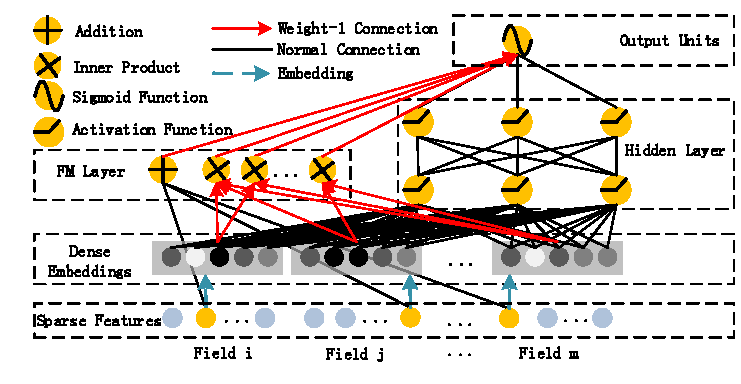
\includegraphics[width=.9\textwidth]{images/architecture-deepfm.pdf}
	\caption{DeepFM}\label{fig:deepfm}
\end{figure}

其主要用于对离散型变量进行训练。
将OneHot编码使用嵌入层嵌入后分别用FM和DNN进行训练,
最终FM和DNN的结果相加后输出。

但是在游戏推荐领域,
往往有非常多的标签数据、
连续型数据例如游玩时间等。
如果使用DeepFM模型,
往往会造成模型过于庞大的问题,
对于大量用户产生的数据,
往往会由于模型复杂度提升而耗费大量的计算资源,
对于对服务器有一定要求的游戏领域往往需要
额外的大量计算资源进行模型的训练。
上述问题均是DeepFM所无法解决的,
因此需要一种新的算法来进行优化,
以尽可能减少计算资源。



\section{系统实验与结果分析}

\subsection{数据处理}

\subsubsection{数据集的来源}

对于游戏推荐算法的研究较少,
数据集的获取也较为困难,
为了兼顾用户数据与游戏数据的广泛性与准确性,
最终选择加利福尼亚大学圣迭戈分校(UCSD)
的Steam游戏数据集
(\url{https://cseweb.ucsd.edu/~jmcauley/datasets.html#steam_data}).

该数据集的基本统计情况如\cref{tb:dataset}所示.

\begin{table}[!htbp]
	\begin{center}
		\caption{Steam数据集基本统计情况}\label{tb:dataset}
		\begin{tabular}{cccc}
			\toprule
			条目 & 数量        & 条目 & 数量     \\
			\midrule
			评论 & 7,793,069 & 项目 & 15,474 \\
			用户 & 2,567,538 & 合集 & 615    \\
			\bottomrule
		\end{tabular}
	\end{center}
\end{table}

\subsubsection{数据的展示}

该数据集主要有五个文件,
分别为澳大利亚用户评论,
澳大利亚用户项目,
合集数据、
Steam游戏数据以及Steam用户评论数据,
均使用Json文件。
本文将仅使用澳大利亚用户相关数据以及游戏相关数据进行训练。

澳大利亚用户评论数据格式不完整展示为:
\begin{minted}[linenos,
		numbersep=5pt,
		frame=lines,
		framesep=2mm]{json}
{
  "reviews": [
    {
      "funny": "",
      "helpful": "No ratings yet",
      "review": "It's unique and worth a playthrough.",
      "recommend": true,
      "item_id": "22200",
      "last_edited": "",
      "posted": "Posted July 15, 2011."
    },
  ],
  "user_id": "76561197970982479",
  "user_url": "http://steamcommunity.com/profiles/
                                    76561197970982479"
}
\end{minted}

澳大利亚用户项目数据格式不完整展示为:
\begin{minted}[linenos,
    numbersep=5pt,
    frame=lines,
    framesep=2mm]{json}
{
  "steam_id": "76561197970982479",
  "items": [
    {
      "item_id": "10",
      "item_name": "Counter-Strike",
      "playtime_2weeks": 0,
      "playtime_forever": 6
    },
  ],
  "items_count": 277,
  "user_id": "76561197970982479",
  "user_url": "http://steamcommunity.com/profiles/
                                    76561197970982479"
}
\end{minted}

游戏数据格式不完整展示为:
\begin{minted}[linenos,
    numbersep=5pt,
    frame=lines,
    framesep=2mm]{json}
{
  "publisher": "Kotoshiro",
  "genres": ["Action", "Casual", "Indie", "Simulation", 
                                                "Strategy"],
  "app_name": "Lost Summoner Kitty",
  "title": "Lost Summoner Kitty",
  "url": "http://store.steampowered.com/app/761140/
                                        Lost_Summoner_Kitty/",
  "release_date": "2018-01-04",
  "tags": ["Strategy", "Action", "Indie", "Casual", 
                                                "Simulation"],
  "discount_price": 4.49,
  "reviews_url": "http://steamcommunity.com/app/761140/
                        reviews/?browsefilter=mostrecent&p=1",
  "id": "761140",
  "price": 4.99,
  "early_access": false,
  "specs": ["Single-player"],
  "developer": "Kotoshiro"
}
\end{minted}

\subsubsection{数据集的预处理}

由于数据集分别包含了评论数据、
用户数据、
游戏数据、
合集数据等.
为了更方便地使用数据集进行训练,
选择将澳大利亚的用户数据、
澳大利亚用户评论数据、
游戏数据进行内连接.

处理之后用于训练的数据不完整展示为:
\begin{minted}[linenos,
    numbersep=5pt,
    frame=lines,
    framesep=2mm]{json}
{
  "game_publisher": "Tripwire Interactive",
  "game_genres": ["Action"],
  "game_name": "Killing Floor",
  "game_title": "Killing Floor",
  "game_release_date": "2009-05-14",
  "game_tags": [
    "FPS", "Zombies", "Co-op",
  ],
  "game_id": "1250",
  "game_price": 19.99,
  "game_earlt_access": false,
  "game_specs": [
    "Single-player", "Multi-player", "Co-op",
  ],
  "game_dev": "Tripwire Interactive",
  "user_id": "76561197970982479",
  "user_steam_id": "76561197970982479",
  "user_items_count": 277,
  "rec": true,
  "review_posted": "Posted November 5, 2011."
}
\end{minted}

鉴于数据集中有一定数据的缺失,
选择将例如游戏制造商、
游戏发行商、
游戏标题等数据填充为\verb|NONE|,
将游戏标签、
游戏风格、
游戏类型等修改为空列表,
游戏价格填充为\verb|0|.

之后对密集数据进行标准化,
标准化的公式为:
\begin{equation}
	\hat{x} = \frac{x-\mu}{\sigma}
\end{equation}

其中$\mu$为数据的平均值,
$\sigma$为数据的方差.

对数据集处理后的可用条目为53,973条.
选择将数据进行8--2划分,
分别作为训练集和验证集.

\subsubsection{Word2Vec到Tag2Vec的迁移}

由于Word2Vec本质上属于是利用上下文数据来进行词嵌入,
对于tag来说可以认为每一条目的标签均为一个句子,
可以根据tag的共现规律进行Word2Vec的训练,
可以很好地解决OneHot编码过于稀疏的问题.
Word2Vec相较于FM等算法其计算性能较高,
可以很好地应用于标签的特征提取.
同时,
对于训练数据而言,
每一条目的标签不多,
不需要设置过大的窗口,
且几乎没有数据的损失.
因此可以作为模型的预训练部分.

\subsection{模型设计\label{sec:design}}

\subsubsection{FM模块设计}

FM模块主要将离散数据分别交给嵌入层和全连接层进行处理,
其中全连接层输出神经元为$1$,
之后将嵌入层的数据交由FM层处理后与线性层结果相加,
最后与嵌入层的数据拼接后输出.
模块的设计主要见\cref{fig:fm}

\begin{figure}[!htbp]
	\centering
	\includegraphics[width=.9\textwidth]{images/fm.pdf}
	\caption{FM模块设计}\label{fig:fm}
\end{figure}

\subsubsection{Word2Vec模块设计}

Word2Vec模块主要在预训练阶段把标签数据进行训练,
对于数据集中的风格、
标签、
类型等信息分别进行训练,
并得出维度为$50$的向量,
对每一相应的标签数据对应的向量相加,
将其作为相应的向量,
拼接后作为输出.

\subsubsection{深度神经网络模块设计}

深度神经网络模块的输入数据为$454$维,
首先将数据通过输出为$454$维的全连接层进行训练,
之后通过维度为$150$的全连接层训练,
第三层则为输出为$50$维的全连接层,
第四层和第五层全连接层的输出维度为$10$和$1$,
为了优化计算性能以及获得较好的训练效果,
全连接层之间的激活函数均选择使用为ReLU,
第五层和输出间的激活函数为Sigmoid.
网络的设计可见\cref{fig:deep}.

\begin{figure}[!htbp]
	\centering
	\includegraphics[width=.9\textwidth]{images/deep.pdf}
	\caption{深度神经网络模块设计}\label{fig:deep}
\end{figure}

\subsection{评价指标}

为了评价建立模型的优劣,
需要建立一个相应的评价体系.
对于本文而言,
其推荐质量的评价主要是通过
对给定数据产生推荐结果的准确性实现.

该推荐算法对游戏的预测主要是对游戏评分的预测,
算法根据用户对游戏评分的多少进行相应的推荐.
因此,
需要一种算法来衡量算法预测评分和用户真实评分的
一种评价指标.
通常的评价指标有:
均方误差损失、
平均绝对值误差损失、
交叉熵损失、
负对数似然函数损失等等.
鉴于该问题适用于二分类问题
(用户评分只有推荐与否),
因此为避免类似于均方误差损失等带来的梯度消失等一系列问题,
因此采用二分类交叉熵损失(BCE).
其计算公式为:
\begin{equation}
	L=-\sum_{i=1}^{N}\left[y_{i} \ln \left(\sigma\left(x_{i}\right)\right)+\left(1-y_{i}\right) \ln \left(1-\sigma\left(x_{i}\right)\right)\right]
\end{equation}

此时有:
\begin{equation}
	\begin{aligned}
		\frac{d L}{d x_{i}} & =\frac{d L}{d \sigma\left(x_{i}\right)} \cdot \frac{d \sigma\left(x_{i}\right)}{d x_{i}}                                                                                         \\
		                    & =-\left[\frac{y_{i}}{\sigma\left(x_{i}\right)}+\left(1-y_{i}\right) \frac{-1}{1-\sigma\left(x_{i}\right)}\right] \sigma\left(x_{i}\right)\left(1-\sigma\left(x_{i}\right)\right) \\
		                    & =\left(\frac{1-y_{i}}{1-\sigma\left(x_{i}\right)}-\frac{y_{i}}{\sigma\left(x_{i}\right)}\right) \sigma\left(x_{i}\right)\left(1-\sigma\left(x_{i}\right)\right)                  \\
		                    & =\left(1-y_{i}\right) \sigma\left(x_{i}\right)-y_{i}\left(1-\sigma\left(x_{i}\right)\right)                                                                                      \\
		                    & =\sigma\left(x_{i}\right)-y_{i}
	\end{aligned}
\end{equation}

其中$ \sigma(x)=\frac{1}{1+e^{-x}} $.

此时可以看到采用Sigmoid作为激活函数与
BCE作为损失函数所得到的梯度值正比于预测值与真实值之差.

\subsection{结果分析}

如前文所述,
对数据集进行训练可以得到训练的结果如\cref{fig:loss}所示.

\begin{figure}[!htbp]
	\centering
	\includegraphics[width=.7\textwidth]{images/loss.pdf}
	\caption{模型损失率曲线}\label{fig:loss}
\end{figure}

由图所示,
伴随迭代周期的增加,
模型的平均损失率在不断减小,
在大约$20$次时趋于收敛.
在第$100$次左右时损失率已经接近$0.17$.
可以看出基本符合预期要求,
同时模型的准确率也能维持在90\%以上的水平,
满足对于推荐所需要的准确率.

\section{总结与展望}

\subsection{本文工作总结}

本文主要基于深度学习相关技术对Steam游戏进行相关的
推荐算法进行研究,
利用神经网络对于特征提取的自动化优势,
融合FM、
Word2Vec等相关技术,
在保证了计算效率的同时兼顾了预测的准确率.
本文的主要工作如下:

首先,
介绍了游戏推荐技术的研究背景以及国内外的研究现状,
对本文的工作提出了一定的可行性分析.
其次,
对相关游戏推荐算法进行了简要的介绍,
对本文即将使用的技术做了铺垫.
之后则对Word2Vec以及FM技术和神经网络技术进行介绍,
扫清了本文的相关技术障碍,
最后对模型进行设计以及训练,
并进行相关结果的分析.

\subsection{未来工作展望}

虽然本文的研究告了一段落,
但是仍然有许多的不足,
例如用户ID,
用户名等没有进行特征提取,
可能会影响到最终模型的性能.
同时对于用户已拥有游戏没有纳入考虑,
由于用户数据集的限制,
无法对用户已拥有游戏的游玩时长进行计算,
造成了大量数据的浪费.
对于用户评论数据,
由于评论语种的限制,
无法对其进行自然语言处理的工作,
如果有一种足够好的语种分类的算法,
可以对其利用TextCNN等一系列NLP处理,
以获得更好的推荐效果.
同时,
可以对用户的评论时间以及评论编辑时间进行相应的处理,
以期获得用户偏好的相应变化.
若能在上述方面取得相应的改进并融合其他推荐算法,
在实际应用中应当能取得较好的结果.

\begin{acknowledge}
    大学四年的时光就要结束了,
    我也即将要步入社会当中,
    回望过去这大学四年,
    我受到了许多人的帮助,
    没有他们,
    也不可能完成这篇毕业设计.

    首先要感谢我的指导老师---黄萍老师,
    在论文的写作期间,
    其给予了我许多宝贵的意见以及写作的指导.
    在黄老师帮指导和帮助下我才得以顺利完成这篇论文.
    同时,
    也要感谢大学四年间所有教过我以及有过接触的老师,
    也正是在他们的教导下,
    不仅学会了专业知识,
    还学会了一些为人处世的道理.

    其次,
    还要感谢QQ群以及微信群的一些网友,
    虽然很多没有见过面也不知道名字,
    但是在我学习编程的道路上给予了我不少的帮助,
    没有他们在这几年的帮助,
    我的代码水平也不足以能够完成本篇的代码编写工作.

    最后,
    还是要感谢几位同学朋友,
    在他们的帮助下坚持学习英语,
    并且在遇到困难的时候得到了他们的帮助.
    没有他们,
    面对大量的英文文献我也不能够流畅的阅读.

    在此,
    我要向所有帮助过我的人表示由衷的谢意,
    祝愿老师们桃李满天下,
    同学朋友们事业有成,
    早日实现奋斗的目标.
\end{acknowledge}

\printbib{}

\end{document}